% arara: pdflatex
% source: http://www.texample.net/tikz/examples/neural-network/
\documentclass[tikz,border=10pt]{standalone}
\usepackage{tikz}
\pagestyle{empty}
\usepackage{arrayjob}

\def\layersep{2.5cm}

\newarray\inputnames
%\readarray{inputnames}{Input 1, Input 2, Input 3, Input 4, Input 5, Input 6,  OC, OHC}     
\def\inputnames{{Input 1, Input 2, Input 3, Input 4, Input 5, Input 6,  OC, OHC}}

\begin{document}
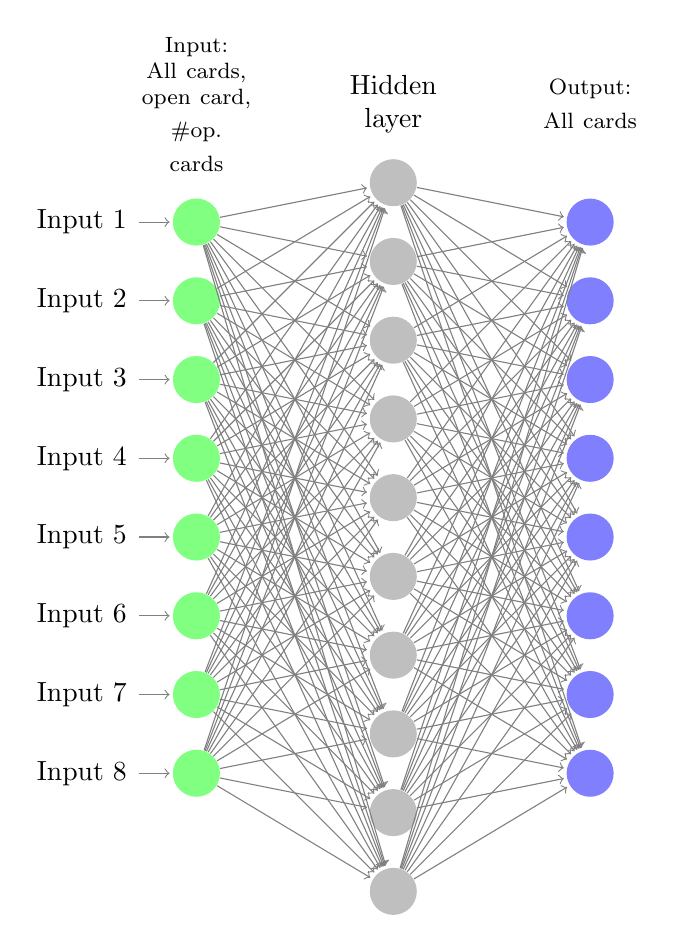
\begin{tikzpicture}[shorten >=1pt,->,draw=black!50, node distance=\layersep]
    \tikzstyle{every pin edge}=[<-,shorten <=1pt]
    \tikzstyle{neuron}=[circle,fill=black!25,minimum size=17pt,inner sep=0pt]
    \tikzstyle{input neuron}=[neuron, fill=green!50];
    \tikzstyle{output neuron}=[neuron, fill=red!50];
    \tikzstyle{hidden neuron}=[neuron, fill=gray!50];
    \tikzstyle{hidden neuron 2}=[neuron, fill=blue!50];
    \tikzstyle{annot} = [text width=4em, text centered]

    % Draw the input layer nodes
    %\foreach \name / \y in {1,...,8}
    \foreach \name / \y in {1,...,8}
        % This is the same as writing \foreach \name / \y in {1/1,2/2,3/3,4/4}
        %\node[input neuron, pin=left:Input \y] (I-\name) at (0,-\y) {};
        \node[input neuron, pin=left: Input \y] (I-\name) at (0,-\y) {};

    % Draw the hidden layer nodes
    \foreach \name / \y in {1,...,10}
        \path[yshift=0.5cm]
            node[hidden neuron] (H1-\name) at (\layersep,-\y cm) {};

    % Draw the hidden output layer
    \foreach \name / \y in {1,...,8}
        \path[yshift=0cm]
        node[hidden neuron 2] (H2-\name) at (\layersep+\layersep,-\y cm) {};


    % Draw the output layer node
    %\node[output neuron,pin={[pin edge={->}]right:Output}, right of=H1-3] (O) {};

    % Connect every node in the input layer with every node in the
    % hidden layer.
    \foreach \source in {1,...,8}
        \foreach \dest in {1,...,10}
            \path (I-\source) edge (H1-\dest);

    \foreach \source in {1,...,10}
        \foreach \dest in {1,...,8}
            \path (H1-\source) edge (H2-\dest);

    % Connect every node in the hidden layer with the output layer
    %\foreach \source in {1,...,10}
        %\path (H1-\source) edge (O);

    % Annotate the layers
    \node[annot,above of=H1-1, node distance=1cm] (hl) {Hidden layer};
    \node[annot,left of=hl] {\footnotesize Input:\\All cards,\\ open card,\\ \#op. cards};
    \node[annot,right of=hl] {\footnotesize Output:\\ All cards};
\end{tikzpicture}
% End of code

\end{document}
